\documentclass[tikz,border=8pt]{standalone}
\usepackage{amsmath}
\usetikzlibrary{arrows.meta,positioning,fit,calc}

\begin{document}
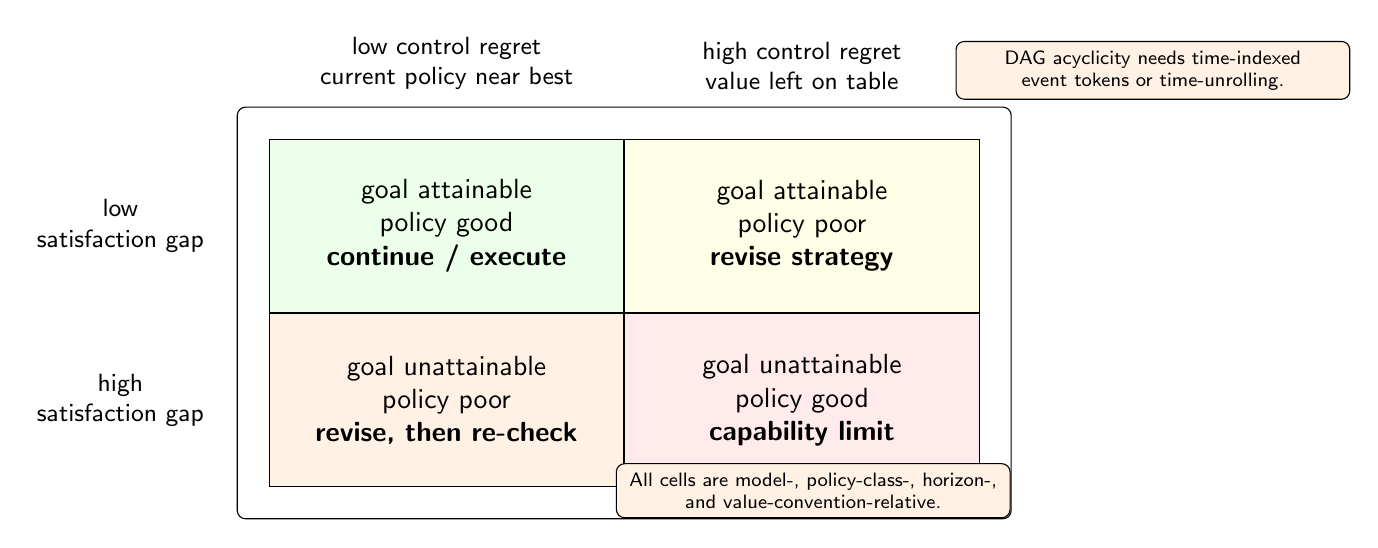
\begin{tikzpicture}[
  font=\sffamily,
  cell/.style={draw, align=center, minimum width=45mm, minimum height=22mm, fill=white},
  label/.style={align=center, font=\sffamily\small},
  warn/.style={draw, rounded corners=3pt, align=center, fill=orange!10, font=\sffamily\scriptsize, minimum width=50mm},
  axis/.style={-Latex, very thick, draw=black!70}
]

\node[cell, fill=green!8] (success) at (0,0) {goal attainable\\policy good\\\textbf{continue / execute}};
\node[cell, fill=yellow!10, right=0mm of success] (regret) {goal attainable\\policy poor\\\textbf{revise strategy}};
\node[cell, fill=orange!10, below=0mm of success] (hardpoor) {goal unattainable\\policy poor\\\textbf{revise, then re-check}};
\node[cell, fill=red!8, below=0mm of regret] (limit) {goal unattainable\\policy good\\\textbf{capability limit}};

\node[label, above=5mm of success] {low control regret\\current policy near best};
\node[label, above=5mm of regret] {high control regret\\value left on table};
\node[label, left=7mm of success] {low\\satisfaction gap};
\node[label, left=7mm of hardpoor] {high\\satisfaction gap};

\node[warn, below=8mm of hardpoor.east, xshift=24mm] (qual)
  {All cells are model-, policy-class-, horizon-,\\and value-convention-relative.};

\node[warn, above=16mm of regret.east, xshift=22mm] (dag)
  {DAG acyclicity needs time-indexed\\event tokens or time-unrolling.};

\node[draw, rounded corners=3pt, fit=(success)(regret)(hardpoor)(limit), inner sep=4mm,
  label={[font=\sffamily\bfseries]below:two signals, four prescriptions}] {};

\end{tikzpicture}
\end{document}
